\begin{figure}[bt!]
  \begin{center}
    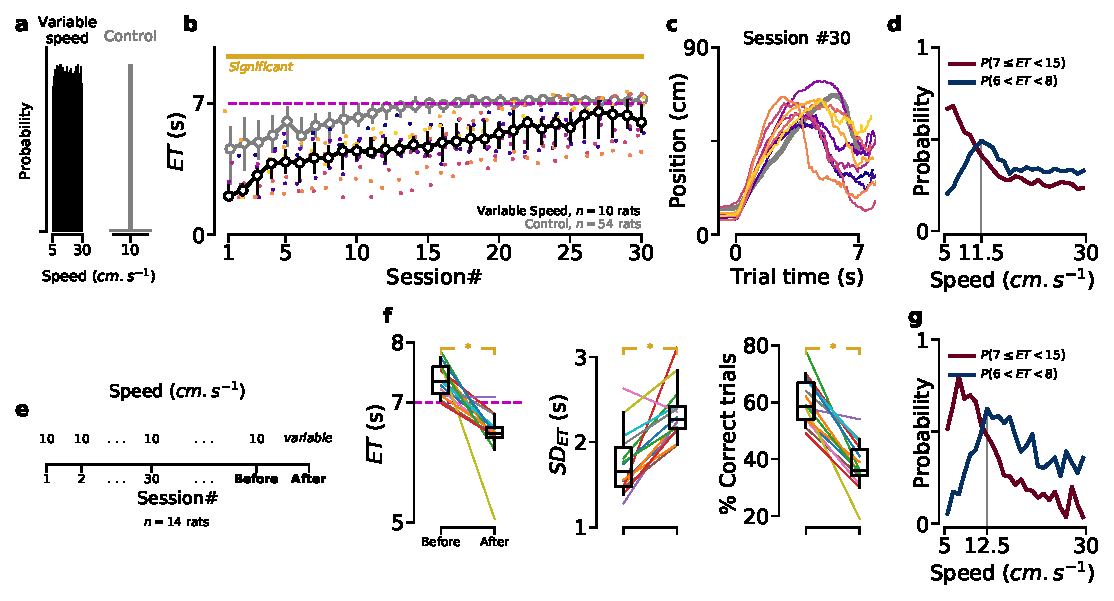
\includegraphics[width=.8\linewidth]{ch-time/figures/VarTrd.pdf}
    \caption[Variable Speed Condition]
    {\textbf{Decreased temporal accuracy when the treadmill speed changes across trials.}
    \textbf{a)}
    For each trial, treadmill speed was either fixed at 10~cm/s (control condition, same data as in \autoref{fig:time:CtrlTrd}), or randomly selected from a uniform distribution between 5 and 30~cm/s (variable speed condition).
    \textbf{b)}
    Median $ET$ for animals trained in the variable speed (black), and control (gray) conditions.
    Colored dots indicate individual performance for ``variable speed'' animals.
    Yellow line shows statistically significant differences between groups (permutation test, see \autoref{ch:methods:tech}).
    \textbf{c)}
    Median trajectory of ``variable speed'' animals in session~\#30 (same colors as in panel~b).
    \textbf{d)}
    Probability of correct ($7\leq~ET<15~s$) and precise ($6<ET<8~s$) trials, given the treadmill speed, for ``variable speed'' animals (session~\# $\geq$20).
    \textbf{e)}
    After extensive training in control condition, animals ($n=14$) were tested in a probe session with variable speed.
    \textbf{f)}
    Median $ET$s (\textit{left}), $SD$ of $ET$s (\textit{middle}) and percentage of correct trials (\textit{right}) in the sessions immediately before and after the change in speed condition.
    Each line represents a single animal.
    Asterisks indicate significant differences (non-parametric paired comparison, see \autoref{ch:methods:tech}).
    \textbf{g)}
    Similar to panel~d, for the data collected from the probe session.
  }
  \label{fig:time:varTrd}
  \end{center}
\end{figure}